\documentclass[a4paper]{article}
\usepackage{indentfirst}
\setlength{\parindent}{2em}
\def\mathbi#1{\textbf{\em #1}}

\usepackage{amsmath} % using math package
\usepackage{amssymb}
\usepackage{cite}
\usepackage{xcolor}
\usepackage{graphicx}

%define new command
\newcommand{\pd}{\partial}


\newcommand{\ket}[1]{\big|  #1 \big \rangle }
\newcommand{\bra}[1]{ \big\langle #1 \big | }

\newcommand {\avg}[3] {\langle {#1} |{ #2} |{#3} \rangle} 

\bibliographystyle{plain} 
\begin{document}
\title{\textbf{Comprehending Quantum mechanics via Stern-Gerlach Experiment}}

\author{Junjie Cai\\\emph{Physics Department,Yunnan University}\\\emph{517924144@qq.com}}
\date{17 Sep, 2018}
\maketitle

Quantum mechanics is a new science developed at the end of the 19th century,which is also used many field,such as quantum communication.Therefore, studying quantum mechanics will help us to learn hot point and forward position field.To comprehend quantum mechanics, we discuss the connect between spin and Stern-Gerlach experiment.


\section{Introduction}
For many people spin is obscure, unlike the physical properties of classical physics. Spin is an intrinsic property of microscopic particle. Otto Stern and Walther Gerlach conducted the Stern-Gerlach experiment in 1922. It was not until 1925 that Ralph Kronig, George Uhlenbeck and Samuel Goudsmit presented the electron spin experiment that Stern-Gerlach experiment obtained a comprehensive explanation. 



In order to facilitate learning, we use Stern-Gerlach experiment to understand quantum state and quantum state superposition.

\section{Stern-Gerlach Experiment}
The experiment used high temperature heating silver atom to make the atom overflow and parallel into rays through the slit to form a thin beam, making it subjected to an inhomogeneous magnetic field produced by a pair of pole pieces, one of which has a very sharp edge. The beam go through a non-uniform magnetic field.The magnetic field $\vec{\mathbi{B}}$ generated by this equipment is basically equipment in the $\mathbi{z}$-direction.And we can learn about that :

\begin{equation} \vec{\mathbi{B}}=\textbf{$B_{\mathbi{z}}$}
\cdot \hat{z}
\end{equation} 

\begin{equation}  
\frac{\partial\vec{\mathbi{B}}}{\partial\hat{\textbf{$\mathbi{z}$}}}\neq  0
\end{equation}
The magnetic field interaction with magnetic moment, causing a potential energy $\textbf{$U_{\mathbi{z}}$}$ :
\begin{equation}
\textbf{$U_{\mathbi{z}}$}=-\vec{\mu}
\cdot\vec{\mathbi{B}}=\textbf{$\mu_{\mathbi{z}}$}
\cdot\textbf{$B_{\mathbi{z}}$}
\end{equation}
The magnetic moment in a non-uniform magnetic field is subject to a force in $\mathcal{Z}$-direction :
\begin{equation}
\textbf{$F_{\mathbi{z}}$}=-\frac{\partial\textbf{$U_{\mathbi{z}}$}}{\partial\textbf{$\mathbi{z}$}}=\textbf{$\mu_{\mathbi{z}}$}
\cdot\frac{\partial\textbf{$B_{\mathbi{z}}$}}{\partial\textbf{$\mathbi{z}$}}
\end{equation}
\begin{figure}[htbp!] \label{figure}
\centering % put the fig. in the center
    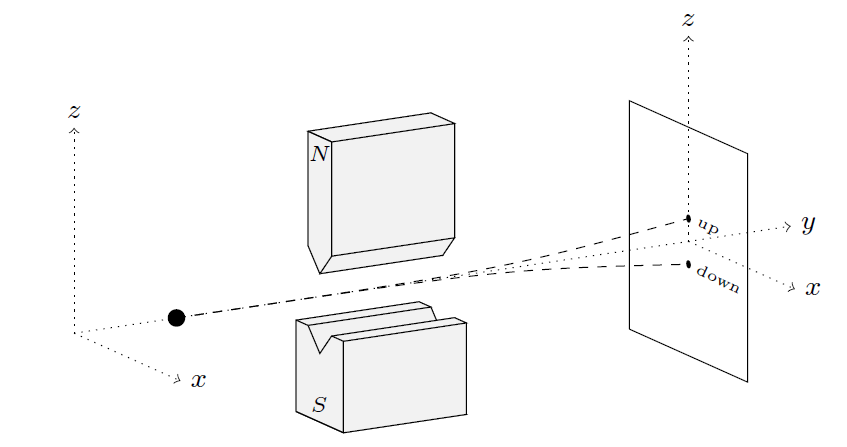
\includegraphics[width=0.8\linewidth]{22.jpg}
    \caption{The experiment of Stern and Gerlach (Adapted from file[1].)}
\end{figure}



Now we consider the atomic magnetic moment of silver, the first nuclear magnetic moment is far less than the magnetic moment of electron, which means that we only need to consider the contribution of electronic magnetic moment of silver atoms, secondly we know to atomic or full filled shells and shell in the contribution of electronic magnetic moment just cancel each other out (orbital magnetic moment and the spin magnetic moment can offset), so that we can determine the atomic magnetic moment of silver mainly from 5$\mathbi{s}$ electronic contribution.we can find the magnetic moment of the silver atom is horizontal, it's not subject to any force, it goes straight through the magnet. If the magnetic moment of an atom is exactly perpendicular, a force pulls it upward toward the sharp magnet. An atom whose magnetic moment is downward will be pushed downward.It
 explains the splitting of the silver atoms in a non-uniform magnetic field\cite{arazo2016stern}.

\section{Sequential Stern-Gerlach Experiment and Polarized Light}
Due to the choice of $\mathbi{z}$-direction is arbitrary, we can assume that the same experiment is also true for non-uniform magnetic fields in the x or y direction, which means that we will find that the silver atoms will split into positive and negative beams of the same proportion in the  $\mathbi{x}$ or $\mathbi{y}$-direction.One consideration is that We regard the whole Stern-Gerlach experiment as an equipment,then We make the silver atoms through a equipment, called \textbf{$SG_{\mathbi{$\hat{z}$}}$} ,getting two beams that split in the $\mathbi{z}$-direction.we can observe two beams independently have two  spin state: $\textbf{$S_{\mathbi{z}}$}$+, $\textbf{$S_{\mathbi{z}}$}$-.
\begin{equation}
\textbf{$S_{\mathbi{z}}$}+=+\frac{1}{2}\hbar, \textbf{$S_{\mathbi{z}}$}-=-\frac{1}{2}\hbar
\end{equation}
Then We block one of these beams($\textbf{$S_{\mathbi{z}}$}$- or $\textbf{$S_{\mathbi{z}}$}$+), getting it through the \textbf{$SG_{\mathbi{z}}$} equipment again, and we find that there is one beam ($\textbf{$S_{\mathbi{z}}$}$+ or $\textbf{$S_{\mathbi{z}}$}$-) it coming out of the second equipment,as show in Figure 2(a).
\begin{figure}[htbp!] \label{figure}
\centering % put the fig. in the center
    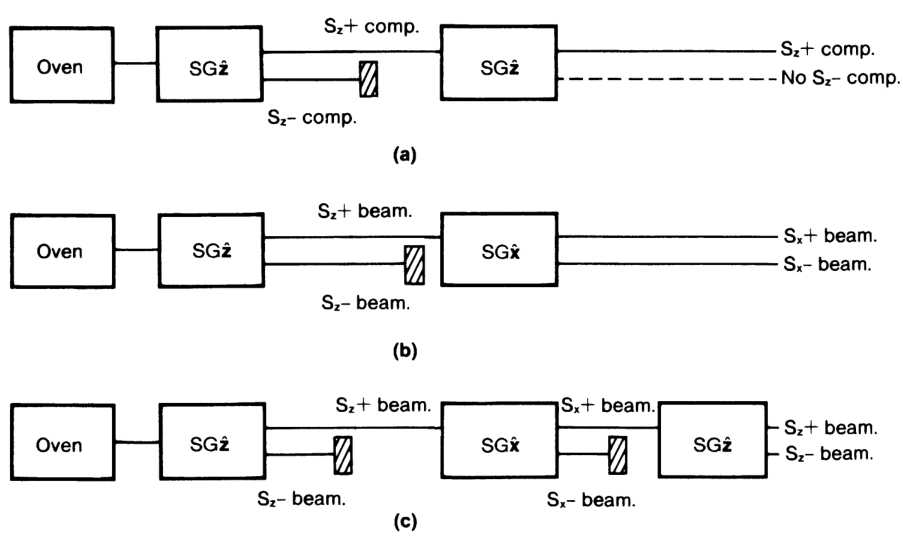
\includegraphics[width=1.0\linewidth]{33.jpg}
    
    \caption{x'- and y'-axes (Adapted from file[2].)}
\end{figure}




We can make the beam $\textbf{$S_{\mathbi{z}}$}$+ continue to pass through an x-direction non-uniform magnetic field (\textbf{$SG_{\mathbi{$\hat{x}$}}$} equipment), and the silver atoms would still split into two beams with a positive and negative 50 percent orientation,as show in Figure 2(b).
However, when we passed the \textbf{$SG_{\mathbi{$\hat{z}$}}$} again, the experimental result is still divided into two beams:$\textbf{$S_{\mathbi{z}}$}$- beam and $\textbf{$S_{\mathbi{z}}$}$+ beam.



This result may be a abstract.We can get this understanding by using the optical analogy.Because light waves are electromagnetic waves, and electromagnetic waves are shear waves, the direction of the oscillations of the electric field component E and the magnetic field component B is perpendicular to the direction of the propagation of the electromagnetic wave.So you have the idea of polarization for electromagnetic waves.We will get  $\mathbi{x}$ -polarized light and  $\mathbi{y}$ -polarized light:

\begin{equation}
\textbf{$\vec{E}_{\mathbi{x}}$}=\textbf{$E_{\mathbi{0}}$}\hat{x}\cos{\left(kz-\omega t\right)}
\end{equation}

\begin{equation}
\textbf{$\vec{E}_{\mathbi{y}}$}=\textbf{$E_{\mathbi{0}}$}\hat{y}\cos{\left(kz-\omega t\right)}
\end{equation}
Polaroid filter can absorb waves that electromagnetic oscillate in a particular direction, such as $\mathbi{x}$ -polaroid absorb energy from all electric fields that are perpendicular to $\mathbi{x}$ -direction, allowing oscillations that are parallel to the direction to penetrate.We can make the transmitted light have a specific polarization direction by rotating the $\mathbi{x}$ direction of the polaroid.
So, for example, we can take an $\mathbi{x}$ -polaroid filter and rotate it counterclockwise 45 degrees to an $\mathbi{x'}$ -polarized light:
\begin{equation}
\textbf{$\vec{E}_{\mathbi{x'}}$}=\frac{\textbf{$E_{\mathbi{0}}$}}{\sqrt{2}}\left(\hat{x}+\hat{y}\right)\cos{\left(kz-\omega t\right)} 
\end{equation}
, and keep rotating 90 degrees to $\mathbi{y'}$ -polarized light:
\begin{equation}
\textbf{$\vec{E}_{\mathbi{y'}}$}=\frac{\textbf{$E_{\mathbi{0}}$}}{\sqrt{2}}\left(-\hat{x}+\hat{y}\right)\cos{\left(kz-\omega t\right)} 
\end{equation}

\begin{figure}[htbp!] \label{figure}
\centering % put the fig. in the center
    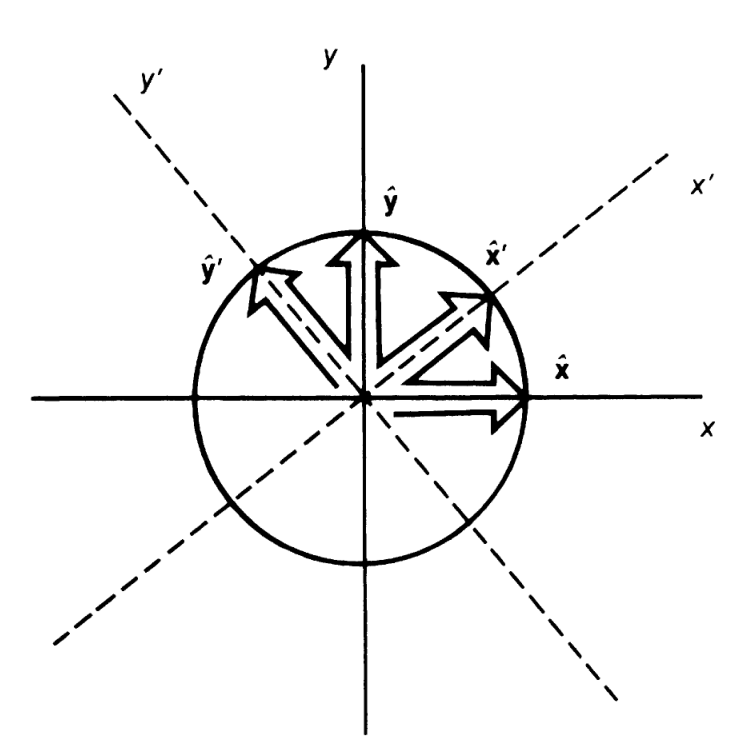
\includegraphics[width=1.0\linewidth]{66.JPG}
    
    \caption{Sequential  Stern-Gerlach  experiments (Adapted from file[2].)}
\end{figure}
Now, we can construct Sequential polaroid filter to make the analogy with the Sequential stern-gallach experiment: first, we make a beam go through the $\mathbi{x}$-polaroid, get the $\mathbi{x}$ -polarized light, make the analogy with sz+, then go on through the$\mathbi{x}$-polaroid, get the $\mathbi{x'}$ -polarized light and make it pass through the $\mathbi{y}$-polaroid,and then we can get $\mathbi{x}$ -polarized light.For X-ray polarized light, electric field in the direction of oscillation in the x direction, x - polarized light through the  $\mathbi{x'}$ -polaroid means perpendicular to the direction of the light will be absorbed, and parallel to the x' will penetrate the direction of the light, electric field intensity of the \textbf{$\vec{E}_{\mathbi{x}}$} is toward projection of the $\mathbi{x'}$ -direction , the factor is $\frac{1}{\sqrt{2}}$. And because of the light intensity is proportional to the square of the electric field intensity, so just 50 percent of the light can penetrate\cite{sakurai1995modern}.
\section{Conclusion}
We can set up a mathematical representation of the quantum state of a silver atom, that is, the spin 1/2 quantum state. We can represent  quantum state which the spin is 1/2 with a two-dimensional column vector corresponding to x-polarized light. We can express \textbf{$S_{\mathbi{z}}$}+ as:
\begin{equation}
\ket{\textbf{$S_{\mathbi{z}}$}+}=\ket{+}=\left( \begin{array}{c} 1 \\ 0 \end{array} \right)
\end{equation}
Similarly, the quantum state \textbf{$S_{\mathbi{z}}$}- is represented by the two-dimensional column vector corresponding to y-polarized light:
\begin{equation}
\ket{\textbf{$S_{\mathbi{z}}$}-}=\ket{-}=\left( \begin{array}{c} 0 \\ 1 \end{array} \right)
\end{equation}
For \textbf{$S_{\mathbi{x}}$}+:
\begin{equation}
\ket{\textbf{$S_{\mathbi{x}}$}+}=\frac{1}{\sqrt{2}}\left( \begin{array}{c} 1 \\ 1 \end{array} \right)
\end{equation}
For \textbf{$S_{\mathbi{x}}$}- :
\begin{equation}
\ket{\textbf{$S_{\mathbi{x}}$}+}=\frac{1}{\sqrt{2}}\left( \begin{array}{c} -1 \\ 1 \end{array} \right)
\end{equation}

\section{Conclusion}


Finally, there are two states$\textbf{$S_{\mathbi{y}}$}\pm$ , which are represented by the two-dimensional column vectors corresponding to circularly polarized light\cite{sakurai1995modern} :
\begin{equation}
\ket{\textbf{$S_{\mathbi{y}}$}+}=\frac{1}{\sqrt{2}}\left( \begin{array}{c} 1 \\ i \end{array} \right),
                           \ket{\textbf{$S_{\mathbi{y}}$}-}=\frac{1}{\sqrt{2}}\left(                     \begin{array}{c} 1 \\ -i \end{array} \right)
\end{equation}
This means that we can represent a spin 1/2 quantum state in a two-dimensional complex coefficient linear vector space.It also helps us understand the concept of spin in quantum mechanics.








\bibliographystyle{IEEEtran}
\bibliography{22}

\end{document}

